% ============================================================================
%  Capítulo 4 - Control GPI (filtrado plano)
% ============================================================================
\chapter{Control proporcional-integral generalizado (GPI)}
\label{cap:GPI}

En este capítulo se construye el controlador GPI usando la teoría de Sira \cite{fliess2002gpi,sira2017adrc},
para la misma dinámica del error del Capítulo~\ref{cap:ADRC-ESO}. Primero se plantea el lazo en forma de fracción,
con la planta y el controlador escritos como cocientes de polinomios, lo que facilita 
entender qué debe tener el controlador para rechazar la perturbación. Después se
construye ese controlador para $n = 1$ usando solo integrales del error y de la
señal de control, sin observador. En la segunda parte se muestra que el ADRC
con ESO es el mismo controlador escrito de otra forma: primero en general y
luego, paso a paso, para $n = 1$ y $m = 1$, con un ESO de orden 2, junto con la
relación entre las ganancias de los dos. Por último, se presenta el caso de estudio del lazo de oxígeno
disuelto en la etapa de lodos activados de una PTAR.

%--------------------------------------------------------------------
\section{Diseño en tiempo continuo}
\label{sec:gpi_continuo}

%--------------------------------------------------------------------
\subsection{Dinámica del error}
\label{subsec:gpi_error}

Se escribe la planta como una función de transferencia
$G(s) = N_G(s)/D_G(s)$ entre la señal de control normalizada,
$u_0 = b_0\,u$, más la perturbación $\bar{\xi}$, y la salida. Con la referencia
$y^{*}$ y el error $e_y = y - y^{*}$:
\begin{align}
y(s) &= \frac{N_G(s)}{D_G(s)}\Bigl[u_0(s) + \bar{\xi}(s)\Bigr] \nonumber\\[4pt]
y(s) - y^{*}(s) &= \frac{N_G(s)}{D_G(s)}\Bigl[u_0(s) + \bar{\xi}(s)\Bigr] - y^{*}(s) \nonumber\\[4pt]
e_y(s) &= \frac{N_G(s)}{D_G(s)}\left[u_0(s) + \bar{\xi}(s) - \frac{D_G(s)}{N_G(s)}\,y^{*}(s)\right] \nonumber\\[4pt]
e_y(s) &= \frac{N_G(s)}{D_G(s)}\Bigl[u_0(s) + \xi(s)\Bigr],
\qquad \xi(s) = \bar{\xi}(s) - \frac{D_G(s)}{N_G(s)}\,y^{*}(s) ,
\end{align}
de modo que
\begin{equation}
e_y(s)\,D_G(s) = N_G(s)\,u_0(s) + N_G(s)\,\xi(s) .
\label{eq:gpi_error_frac}
\end{equation}
Como en \eqref{eq:error_n}, la referencia queda dentro de la perturbación total:
para la cadena de integradores, $G(s) = 1/s^n$, el término
$\bigl(D_G(s)/N_G(s)\bigr)\,y^{*}(s) = s^n y^{*}(s)$ es la señal $u^{*} = y^{*(n)}$, y
$\xi = \bar{\xi} - u^{*}$, es decir, $u^{*}$ es lo que $u$ debe compensar por introducir la referencia en la perturbación.

%--------------------------------------------------------------------
\subsection{Ley de control y lazo cerrado}
\label{subsec:gpi_lazo}

El controlador se escribe también como fracción, separando los polos que quedan en el origen:
\begin{equation}
u_0(s) = \left[\frac{N_C(s)}{s^{m}\,\bar{D}_C(s)}\right]\bigl(-e_y(s)\bigr),
\qquad D_A(s) := s^{m} .
\label{eq:gpi_ley_general}
\end{equation}
$D_A$ es el modelo interno de la perturbación: una perturbación polinomial de
grado $m - 1$ en el tiempo es eliminada, o aniquilada, totalmente del sistema, en el mismo sentido
del modelo interno de orden $m$ del Capítulo~\ref{cap:ADRC-ESO}. Ahora bien,
sustituyendo la $u_0$ de \eqref{eq:gpi_ley_general} en \eqref{eq:gpi_error_frac}:
\begin{align}
e_y(s)\,D_G(s) &= N_G(s)\left[\frac{N_C(s)}{D_A(s)\,\bar{D}_C(s)}\right]\bigl(-e_y(s)\bigr) + N_G(s)\,\xi(s) \nonumber\\[4pt]
e_y(s)\,D_G(s) &= \frac{-N_G(s) N_C(s)\,e_y(s) + D_A(s) \bar{D}_C(s) N_G(s)\,\xi(s)}{D_A(s) \bar{D}_C(s)} \nonumber\\[4pt]
e_y(s)\,D_G(s) D_A(s) \bar{D}_C(s) + N_C(s) N_G(s)\,e_y(s) &= D_A(s) \bar{D}_C(s) N_G(s)\,\xi(s) ,
\end{align}
\begin{equation}
\begin{gathered}
\boxed{\;\bigl[D_G(s) \bar{D}_C(s) D_A(s) + N_C(s) N_G(s)\bigr]\,e_y(s) = D_A(s) \bar{D}_C(s) N_G(s)\,\xi(s)\;}\\[4pt]
P(s) := D_G(s) \bar{D}_C(s) D_A(s) + N_C(s) N_G(s) .
\end{gathered}
\label{eq:gpi_lazo_general}
\end{equation}
$P(s)$ es el polinomio característico del lazo cerrado, el que da la dinámica del
error de seguimiento, y el cociente es la
función de sensibilidad en lazo cerrado del sistema, que traduce el efecto de
la perturbación sobre el error \cite{sira2017adrc}. Se le pone el
subíndice $\xi$, $S_{\xi}$, porque es la sensibilidad frente a la perturbación
total, para no confundirla con la sensibilidad $S(s)$ de \eqref{eq:mapa_robustez}:
\begin{equation}
e_y(s) = S_{\xi}(s)\,\xi(s), \qquad
S_{\xi}(s) = \frac{D_A(s)\,\bar{D}_C(s)\,N_G(s)}{P(s)} .
\label{eq:gpi_sensibilidad}
\end{equation}
Si la perturbación es, o se aproxima por tramos a, una señal de grado $m - 1$ en el tiempo, su
derivada $m$-ésima es cero, y eso es justo lo que hace el $s^{m}$ de $D_A(s)$ en el numerador de
$S_{\xi}(s)$: aniquila la perturbación. Si además $P(s)$ es Hurwitz y la perturbación es anulada, el
error tiende a cero \eqref{eq:gpi_lazo_general}, y si la aproximación es solo por tramos, queda
pequeño. Por ejemplo, para una perturbación constante ($m = 1$, grado $0$ en el tiempo),
$\xi(s) = \xi(\infty)/s$ y $D_A(s) = s$, y con el teorema del valor final tendríamos:
\begin{equation}
\lim_{t\to\infty} e_y(t) = \lim_{s\to 0} s\,S_{\xi}(s)\,\frac{\xi(\infty)}{s}
= S_{\xi}(0)\,\xi(\infty) = 0 ,
\label{eq:gpi_valor_final}
\end{equation}
que es cero porque el $s$ de $D_A(s)$ pone un cero de $S_{\xi}(s)$ en el origen. El diseño
consiste entonces en escoger $N_C(s)$ y $\bar{D}_C(s)$ para que $P(s)$ tenga las raíces
deseadas, es decir, que la dinámica del error la definamos nosotros, y en escoger un $D_A(s)$ que
permita aniquilar o eliminar la perturbación.

%--------------------------------------------------------------------
\subsection{Construcción del controlador con integradores}
\label{subsec:gpi_integradores}
Se construye el controlador para la planta de primer orden, $n = 1$,
\begin{equation}
\dot{e}_y(t) = u_0(t) + \xi(t) ,
\label{eq:gpi_planta}
\end{equation}
usando solo $e_y$, $u_0$ y sus integrales: no hay derivadas ni observador. Como la orden
real es $u = u_0/b_0$, la planta de diseño vista desde $u$ es $b_0/s$ y el controlador completo
es $C(s)$; en el lazo los dos van multiplicados, $C(s)\,b_0/s$, y el $b_0$ de la planta se
cancela con el $1/b_0$ del controlador. Por eso lo que se diseña es $b_0\,C(s)$, de $-e_y$ a
$u_0$, con ganancias que no dependen de $b_0$, y $b_0$ solo vuelve a aparecer al final, al
pasar de $u_0$ a $u$. Las ganancias se numeran de forma que el subíndice coincida con la potencia de $s$
que multiplican en el polinomio característico. Su análisis se hizo de forma inductiva,
viendo patrones a medida que cambiamos la forma del controlador, por ejemplo:

\paragraph{A. Solo proporcional.}
\begin{equation}
u_0(t) = -k_0\,e_y(t)
\quad\Longrightarrow\quad
e_y(s)\,(s + k_0) = \xi(s)
\quad\Longrightarrow\quad
e_y(s) = \frac{\xi(s)}{s + k_0} .
\end{equation}
Con el teorema del valor final, como en \eqref{eq:gpi_valor_final} pero sin el
cero de $D_A$ en $S_{\xi}(s)$, el error final es $S_{\xi}(0)\,\xi(\infty) = \xi(\infty)/k_0 \neq 0$:
queda un error de estado estacionario porque falta el modelo interno de $\xi$
($m = 0$, no hay $D_A$).

\paragraph{B. Proporcional más integral (GPI mínimo).}
\begin{equation}
u_0(t) = -k_1\,e_y(t) - k_0\!\int_0^t\! e_y(\tau)\,d\tau
\quad\Longrightarrow\quad
s\,e_y(s) + k_1 e_y(s) + \frac{k_0}{s}\,e_y(s) = \xi(s) ,
\label{eq:gpi_pi}
\end{equation}
\begin{equation}
e_y(s)\bigl[s^2 + k_1 s + k_0\bigr] = s\,\xi(s)
\quad\Longrightarrow\quad
\lim_{t\to\infty} e_y(t) = 0 .
\end{equation}
La $s$ del lado derecho es el integrador del controlador, $D_A = s$: es lo que
anula una $\xi$ constante. Esto ya funciona, y es un PI clásico bipropio,
$b_0\,C(s) = (k_1 s + k_0)/s$.

\paragraph{C. Reemplazar la medida por una reconstrucción.} Para $n = 1$ el error se mide y no hace
falta reconstruirlo para conocerlo, pero reconstruirlo es lo que lleva al ESO, que también estima $e_y$
aunque se mida, y agrega un filtrado del ruido de la medida. Se busca reconstruir la
señal del error de seguimiento $e_y$ en términos de la señal de control, para usarla
en \eqref{eq:gpi_pi}. Para ello, integrando una vez la planta \eqref{eq:gpi_planta},
\begin{equation}
\begin{gathered}
\int_0^t\!\dot{e}_y(\tau)\,d\tau = \int_0^t\! u_0(\tau)\,d\tau + \int_0^t\! \xi(\tau)\,d\tau \\
\Longrightarrow\quad
e_y(t) = \int_0^t\! u_0(\tau)\,d\tau + \textcolor{red}{\int_0^t\! \xi(\tau)\,d\tau + e_y(0)} .
\end{gathered}
\end{equation}
Quitando lo desconocido, $e_y(0)$ y $\xi$, queda el reconstructor integral de
la salida,
\begin{equation}
\hat{e}_y(t) = \int_0^t\! u_0(\tau)\,d\tau .
\label{eq:gpi_reconstructor}
\end{equation}
Lo que se quitó, en rojo, es el residuo de la reconstrucción: un residuo tipo
constante, $e_y(0)$, por la condición inicial, y uno tipo rampa,
$\int_0^t \xi(\tau)\,d\tau$, que para una $\xi$ constante crece como $\xi\,t$. Al
suponer el error como en \eqref{eq:gpi_reconstructor}, ese residuo no se ve, y va
a tener que ser compensado después con integrales del error.
Si se realimenta esa reconstrucción en lugar del error medido, se tiene el siguiente controlador:
\begin{equation}
\begin{gathered}
u_0(t) = -k_1\!\int_0^t\! u_0(\tau)\,d\tau - k_0\!\int_0^t\! e_y(\tau)\,d\tau \\
\Longrightarrow\quad
u_0(s)\Bigl(1 + \frac{k_1}{s}\Bigr) = -\frac{k_0}{s}\,e_y(s)
\quad\Longrightarrow\quad
u_0(s) = -\frac{k_0}{s + k_1}\,e_y(s) ,
\end{gathered}
\end{equation}
\begin{equation}
e_y(s)\bigl[s^2 + k_1 s + k_0\bigr] = (s + k_1)\,\xi(s)
\quad\Longrightarrow\quad
\lim_{t\to\infty} e_y(t) = \frac{k_1\,\xi(\infty)}{k_0} \neq 0 .
\end{equation}
No se cumple: la integral de $u_0$ llevó el $1/s$ al denominador, así que
$b_0\,C(s) = k_0/(s + k_1)$ no tiene polo en el origen, y el integrador que antes rechazaba
$\xi$ se gastó en el reconstructor. Si bien la integral del error,
con $k_0$, elimina el residuo tipo constante $e_y(0)$, el residuo tipo rampa de
$\int \xi$ queda sin compensar, y de ahí el error final $k_1\,\xi(\infty)/k_0$, por lo que es necesario
compensarlo agregando más integradores.

\paragraph{D. Una integral más del error.} Para compensar
también el residuo tipo rampa se agrega una integral más del error, y con ella la
ganancia $k_2$; las ganancias se reorganizan para que tengan un orden relacionado con el
polinomio característico, es decir, se renombran para que el subíndice siga coincidiendo
con la potencia de $s$:
\begin{equation}
u_0(t) = -k_2\!\int_0^t\! u_0(\tau)\,d\tau - k_1\!\int_0^t\! e_y(\tau)\,d\tau
- k_0\!\iint e_y(\tau)\,d\tau ,
\label{eq:gpi_integrales}
\end{equation}
\begin{equation}
u_0(s) = -\frac{k_2}{s}\,u_0(s) - \frac{k_1}{s}\,e_y(s) - \frac{k_0}{s^2}\,e_y(s)
\quad\Longrightarrow\quad
u_0(s)\Bigl(1 + \frac{k_2}{s}\Bigr) = -\frac{k_1 s + k_0}{s^2}\,e_y(s) ,
\end{equation}
\begin{equation}
\boxed{\;u_0(s) = -\frac{k_1 s + k_0}{s\,(s + k_2)}\,e_y(s)\;}
\label{eq:gpi_ley}
\end{equation}
Cerrando el lazo con \eqref{eq:gpi_planta},
\begin{equation}
\begin{gathered}
s\,e_y(s) = -\frac{k_1 s + k_0}{s\,(s + k_2)}\,e_y(s) + \xi(s) \\
\Longrightarrow\quad
s\,e_y(s)\,s\,(s + k_2) + (k_1 s + k_0)\,e_y(s) = s\,(s + k_2)\,\xi(s) ,
\end{gathered}
\end{equation}
\begin{equation}
e_y(s)\bigl[s^3 + k_2 s^2 + k_1 s + k_0\bigr] = s\,(s + k_2)\,\xi(s)
\quad\Longrightarrow\quad
\lim_{t\to\infty} e_y(t) = 0 .
\label{eq:gpi_cerrado}
\end{equation}
El error tiende a cero solo si la señal de entrada, la perturbación $\xi$, es tipo constante, $1/s$
en Laplace.

\paragraph{Conteo de integradores.} En general, para una planta de orden
$n$ (la cadena de $n$ integradores) y una perturbación polinomial de grado $m - 1$ en el tiempo,
con $m$ polos en el origen, la ley lleva integrales de $u_0$ hasta de orden $n$, que reconstruyen el
error y sus derivadas, e integrales del error hasta de orden $n + m$. En Laplace,
las de $u_0$ quedan en el denominador y las del error en el numerador:
\begin{equation}
b_0\,C(s) = \frac{N_C(s)}{s^{m}\,\bar{D}_C(s)} ,
\qquad \operatorname{grado} \bar{D}_C = n ,
\qquad \operatorname{grado} N_C = n + m - 1 ,
\label{eq:gpi_integradores_netos}
\end{equation}
así van a quedar $m$ integradores, los de $D_A = s^{m}$, que corresponden al modelo interno. Con
$G(s) = 1/s^{n}$, el polinomio característico $P(s) = s^{n+m}\bar{D}_C(s) + N_C(s)$ tiene grado
$2n + m$, y el controlador tiene justo $2n + m$ ganancias, una por cada raíz que se quiere ubicar; es
decir, manteniendo este orden siempre se pueden escoger las ganancias para que $P(s)$ sea Hurwitz. La
Tabla~\ref{tab:gpi_conteo} muestra lo que cambia al subir el orden de la planta o
de la perturbación.

\begin{table}[H]
\centering
\caption[Integradores del GPI según la planta y la perturbación]{Controlador GPI
  \eqref{eq:gpi_integradores_netos} para una planta de orden $n$ y una
  perturbación modelada como la salida de $m$ integradores, $1/s^{m}$ en Laplace (un
  polinomio de grado $m - 1$ en el tiempo): orden de las integrales de $u_0$ y
  del error, y grado de $P(s)$, que es también el número de ganancias. Las
  ganancias se numeran con la potencia de $s$ que multiplican en $P(s)$. En
  negrita, el caso de este trabajo.}
\label{tab:gpi_conteo}
\small
\renewcommand{\arraystretch}{2.2}
\setlength{\tabcolsep}{4.5pt}
\begin{tabular}{ccccc}
\toprule
\textbf{Planta} & \textbf{Perturbación} & $b_0\,C(s)$ & \textbf{Integrales} $u_0$ / $e_y$ & \textbf{Grado de} $P(s)$ \\
\midrule
$\mathbf{n = 1}$ & \textbf{constante} ($\mathbf{m = 1}$) & $\dfrac{k_1 s + k_0}{s\,(s + k_2)}$ & $\mathbf{1}$ / $\mathbf{2}$ & $\mathbf{3}$ \\
$n = 1$ & rampa ($m = 2$) & $\dfrac{k_2 s^2 + k_1 s + k_0}{s^2\,(s + k_3)}$ & $1$ / $3$ & $4$ \\
$n = 2$ & constante ($m = 1$) & $\dfrac{k_2 s^2 + k_1 s + k_0}{s\,(s^2 + k_4 s + k_3)}$ & $2$ / $3$ & $5$ \\
$n = 2$ & rampa ($m = 2$) & $\dfrac{k_3 s^3 + k_2 s^2 + k_1 s + k_0}{s^2\,(s^2 + k_5 s + k_4)}$ & $2$ / $4$ & $6$ \\
\midrule
$n$ & polinomio ($m$) & $\dfrac{\sum_{i=0}^{n+m-1} k_i\,s^{i}}{s^{m}\,\bigl(s^{n} + \sum_{i=0}^{n-1} k_{n+m+i}\,s^{i}\bigr)}$ & $n$ / $n + m$ & $2n + m$ \\
\bottomrule
\end{tabular}
\end{table}

%--------------------------------------------------------------------
\subsection{Caso de primer orden en la forma general}
\label{subsec:gpi_primer_orden}

El controlador \eqref{eq:gpi_ley} es un caso de \eqref{eq:gpi_ley_general}, con
\begin{equation}
\begin{gathered}
n = 1,\quad G(s) = \frac{1}{s}\;\bigl(N_G(s) = 1,\ D_G(s) = s\bigr),\quad
m = 1\;\bigl(D_A(s) = s\bigr),\\[4pt]
N_C(s) = k_1 s + k_0,\quad \bar{D}_C(s) = s + k_2 .
\end{gathered}
\end{equation}
Sustituyendo en \eqref{eq:gpi_lazo_general} se llega al mismo lazo cerrado
\eqref{eq:gpi_cerrado}:
\begin{align}
\bigl[D_G(s) \bar{D}_C(s) D_A(s) + N_C(s) N_G(s)\bigr]\,e_y(s) &= D_A(s) \bar{D}_C(s) N_G(s)\,\xi(s) \nonumber\\[4pt]
\bigl[s\,\bar{D}_C(s)\,s + N_C(s)\bigr]\,e_y(s) &= s\,\bar{D}_C(s)\,\xi(s) \nonumber\\[4pt]
\bigl[s^2\,(s + k_2) + k_1 s + k_0\bigr]\,e_y(s) &= s\,(s + k_2)\,\xi(s) \nonumber\\[4pt]
\bigl[s^3 + k_2 s^2 + k_1 s + k_0\bigr]\,e_y(s) &= s\,(s + k_2)\,\xi(s) ,
\end{align}
con la función de sensibilidad en lazo cerrado
\begin{equation}
S_{\xi}(s) = \frac{s\,(s + k_2)}{s^3 + k_2 s^2 + k_1 s + k_0} , \qquad S_{\xi}(0) = 0 .
\label{eq:gpi_S}
\end{equation}

%--------------------------------------------------------------------
\section{Relación con el ESO}
\label{sec:gpi_eso}

%--------------------------------------------------------------------
\subsection{Forma general}
\label{subsec:gpi_eso_general}

El observador \eqref{eq:observador} del Capítulo~\ref{cap:ADRC-ESO} es
\begin{equation}
\dot{\widehat{\mathbf{X}}}(t) = \bigl(\mathbf{A} - \mathbf{L}\mathbf{C}\bigr)\widehat{\mathbf{X}}(t)
+ \mathbf{B}\,u_0(t) + \mathbf{L}\,e_y(t) .
\end{equation}
El observador solo ve la cadena de integradores, porque el sistema aumentado
solo contiene esa dinámica; por eso $b_0$ no entra en el observador, sino al
final, en $u(t) = u_0(t)/b_0$. Con la ley de control \eqref{eq:ley_matricial},
$u_0(t) = -\mathbf{K}\,\widehat{\mathbf{X}}(t)$, el observador queda con una sola
entrada, el error:
\begin{equation}
\dot{\widehat{\mathbf{X}}}(t) = \bigl(\mathbf{A} - \mathbf{L}\mathbf{C} - \mathbf{B}\mathbf{K}\bigr)\widehat{\mathbf{X}}(t)
+ \mathbf{L}\,e_y(t) ,
\end{equation}
que es un sistema en espacio de estados con
\begin{equation}
\mathbf{A}_c = \mathbf{A} - \mathbf{L}\mathbf{C} - \mathbf{B}\mathbf{K},\quad
\mathbf{B}_c = \mathbf{L}_{(n+m)\times 1},\quad
\mathbf{C}_c = \mathbf{I}_{(n+m)\times(n+m)},\quad
\mathbf{D}_c = \mathbf{0}_{(n+m)\times 1} .
\end{equation}
Su función de transferencia es un vector, una entrada por cada estado estimado:
\begin{equation}
\frac{\widehat{\mathbf{X}}(s)}{e_y(s)} = \mathbf{G}_X(s)
= \mathbf{C}_c\bigl[s\mathbf{I} - \mathbf{A}_c\bigr]^{-1}\mathbf{B}_c + \mathbf{D}_c
= \begin{bmatrix} G_{X_1}(s) \\ G_{X_2}(s) \\ \vdots \\ G_{X_{n+m}}(s) \end{bmatrix} ,
\end{equation}
y la ley de control la reduce a un escalar:
\begin{equation}
u(s) = -\frac{1}{b_0}\,\mathbf{K}_{1\times(n+m)}\,\mathbf{G}_X(s)_{(n+m)\times 1}\,e_y(s)
\quad\Longrightarrow\quad
b_0\,C(s) = \mathbf{K}\bigl[s\mathbf{I} - \mathbf{A}_c\bigr]^{-1}\mathbf{L} .
\label{eq:gpi_eso_general}
\end{equation}
Este $C(s)$ es una fracción de polinomios y tiene la forma
\eqref{eq:gpi_ley_general}. Para $m = 1$, la columna de $\mathbf{A}_c$ que
corresponde a $\hat{\xi}$ queda en ceros: en $\mathbf{A}$ esa columna solo tiene
el $1$ que conecta la perturbación con la última derivada, y $\mathbf{B}\mathbf{K}$
pone ahí el $1$ que la cancela. Por eso $\det(s\mathbf{I} - \mathbf{A}_c)$ tiene
el factor $s$, que es el $D_A = s$ de la forma general: el integrador del
controlador es el estado $\hat{\xi}$.

%--------------------------------------------------------------------
\subsection{Paso a paso para $n = 1$, $m = 1$}
\label{subsec:gpi_eso_tf}

Con un ESO de orden 2, las matrices del modelo de diseño (cadena de integradores
y perturbación constante) y las ganancias son
\begin{equation}
\mathbf{A} = \begin{bmatrix} 0 & 1 \\ 0 & 0 \end{bmatrix},\quad
\mathbf{B} = \begin{bmatrix} 1 \\ 0 \end{bmatrix},\quad
\mathbf{C} = \begin{bmatrix} 1 & 0 \end{bmatrix},\quad
\mathbf{L} = \begin{bmatrix} l_1 \\ l_2 \end{bmatrix},\quad
\mathbf{K} = \begin{bmatrix} k_{p_1} & 1 \end{bmatrix} ,
\end{equation}
con $\widehat{\mathbf{X}}(t) = [\hat{e}_y(t) \;\; \hat{\xi}(t)]^{\top}$. La segunda entrada
de $\mathbf{K}$ es el $1$ que cancela $\hat{\xi}$ en la ley de control.

\paragraph{Matriz del observador en lazo cerrado.}
\begin{equation}
\mathbf{A}_c =
\underbrace{\begin{bmatrix} 0 & 1 \\ 0 & 0 \end{bmatrix}}_{\mathbf{A}}
-\underbrace{\begin{bmatrix} l_1 \\ l_2 \end{bmatrix}\begin{bmatrix} 1 & 0 \end{bmatrix}}_{\mathbf{L}\mathbf{C}}
-\underbrace{\begin{bmatrix} 1 \\ 0 \end{bmatrix}\begin{bmatrix} k_{p_1} & 1 \end{bmatrix}}_{\mathbf{B}\mathbf{K}}
= \begin{bmatrix} 0 & 1 \\ 0 & 0 \end{bmatrix}
- \begin{bmatrix} l_1 & 0 \\ l_2 & 0 \end{bmatrix}
- \begin{bmatrix} k_{p_1} & 1 \\ 0 & 0 \end{bmatrix} ,
\end{equation}
\begin{equation}
\mathbf{A}_c = \begin{bmatrix} -(k_{p_1} + l_1) & 0 \\ -l_2 & 0 \end{bmatrix} .
\end{equation}
El $1$ de $\mathbf{A}$ y el $1$ de $\mathbf{B}\mathbf{K}$ se cancelan, por eso
la entrada $(1,2)$ es cero: es la columna nula de la forma general.

\paragraph{Resolvente.} Al restar $\mathbf{A}_c$ cambian de signo todas las entradas:
\begin{equation}
s\mathbf{I} - \mathbf{A}_c = \begin{bmatrix} s + k_{p_1} + l_1 & 0 \\ l_2 & s \end{bmatrix},
\qquad
\det\bigl(s\mathbf{I} - \mathbf{A}_c\bigr) = s\,(s + k_{p_1} + l_1) ,
\end{equation}
\begin{equation}
\bigl[s\mathbf{I} - \mathbf{A}_c\bigr]^{-1} = \frac{1}{s\,(s + k_{p_1} + l_1)}
\begin{bmatrix} s & 0 \\ -l_2 & s + k_{p_1} + l_1 \end{bmatrix} .
\end{equation}

\paragraph{Estados en función del error.} Como $\mathbf{B}_c = \mathbf{L}$, el
resolvente multiplica el vector de ganancias fila por fila:
\begin{equation}
\mathbf{G}_X(s) = \bigl[s\mathbf{I} - \mathbf{A}_c\bigr]^{-1}\mathbf{L}
= \frac{1}{s\,(s + k_{p_1} + l_1)}
\begin{bmatrix} s & 0 \\ -l_2 & s + k_{p_1} + l_1 \end{bmatrix}
\begin{bmatrix} l_1 \\ l_2 \end{bmatrix} ,
\end{equation}
\begin{equation}
\mathbf{G}_X(s)
= \frac{1}{s\,(s + k_{p_1} + l_1)}
\begin{bmatrix} s\cdot l_1 + 0\cdot l_2 \\ -l_2\cdot l_1 + (s + k_{p_1} + l_1)\,l_2 \end{bmatrix}
= \frac{1}{s\,(s + k_{p_1} + l_1)}
\begin{bmatrix} l_1\,s \\ l_2\,(s + k_{p_1}) \end{bmatrix} .
\end{equation}
En la segunda fila, el $-l_1 l_2$ se cancela con el $+l_1 l_2$ del producto, y
queda $l_2(s + k_{p_1})$.

\paragraph{Ley de control.} Con
$u(t) = -\frac{1}{b_0}\mathbf{K}\,\widehat{\mathbf{X}}(t) = -\frac{1}{b_0}\bigl(k_{p_1}\hat{e}_y(t) + \hat{\xi}(t)\bigr)$,
\eqref{eq:gpi_eso_general} da la función de transferencia de $-e_y$ a $u_0$:
\begin{equation}
b_0\,C(s) = k_{p_1}\frac{l_1\,s}{s\,(s + k_{p_1} + l_1)} + \frac{l_2\,(s + k_{p_1})}{s\,(s + k_{p_1} + l_1)}
= \frac{(k_{p_1} l_1 + l_2)\,s + k_{p_1} l_2}{s\,(s + k_{p_1} + l_1)} ,
\label{eq:gpi_eso_tf}
\end{equation}
que tiene la forma del filtro plano \eqref{eq:gpi_ley}, con
$D_A = s$, $\bar{D}_C = s + k_{p_1} + l_1$ y $N_C = (k_{p_1} l_1 + l_2)\,s + k_{p_1} l_2$.

%--------------------------------------------------------------------
\subsection{Relación entre las ganancias}
\label{subsec:gpi_eso_ganancias}

Igualando \eqref{eq:gpi_eso_tf} con \eqref{eq:gpi_ley}, las ganancias del GPI
se leen directamente de las del ESO:
\begin{equation}
\boxed{\;k_2 = k_{p_1} + l_1, \qquad k_1 = k_{p_1} l_1 + l_2, \qquad k_0 = k_{p_1} l_2\;}
\label{eq:eso2gpi}
\end{equation}
Con estos $N_C$ y $\bar{D}_C$, el polinomio $P(s)$ de \eqref{eq:gpi_lazo_general} es
un producto de polinomios:
\begin{equation}
P(s) = s^3 + k_2 s^2 + k_1 s + k_0
= \underbrace{(s + k_{p_1})}_{p_c(s)}\,\underbrace{(s^2 + l_1 s + l_2)}_{p_o(s)} .
\label{eq:gpi_producto}
\end{equation}
Es el principio de separación \eqref{eq:separacion} visto desde el GPI: el
polinomio característico es el producto del polinomio del
controlador, $p_c(s)$, y el del observador, $p_o(s)$
\cite{sira2017adrc}. Con \eqref{eq:gpi_S}, la función de
sensibilidad en lazo cerrado del ADRC queda
\begin{equation}
S_{\xi}(s) = \frac{s\,(s + k_{p_1} + l_1)}{(s + k_{p_1})\,(s^2 + l_1 s + l_2)} ,
\label{eq:gpi_producto_S}
\end{equation}
con el cero en el origen que rechaza $\xi$ constante. El polinomio
característico y los ceros de $e_y/\xi$ coinciden, así que es el mismo
controlador. Sin la $s$ del denominador de
\eqref{eq:gpi_eso_tf} el controlador no tendría integrador y una $\xi$ constante
no se rechazaría.

La Tabla~\ref{tab:gpi_eso} resume la relación con los valores del caso PTAR
($k_{p_1} = \omega_c$, $l_1 = 2\omega_o$, $l_2 = \omega_o^2$;
Tabla~\ref{tab:caso_parametros}).

\begin{table}[H]
\centering
\caption[Relación entre las ganancias del ESO y del GPI]{Relación entre las
ganancias del ADRC con ESO de orden 2 ($n = m = 1$) y las del GPI
\eqref{eq:gpi_ley}. Los valores numéricos son los del caso PTAR, con
$\omega_c = 3{,}33\times10^{-3}$~rad/s y $\omega_o = 5\,\omega_c$; entre
paréntesis, el controlador en las unidades de la planta, dividido por
$b_0 = 4{,}17\times10^{-5}$.}
\label{tab:gpi_eso}
\begin{tabular}{@{}llll@{}}
\toprule
GPI & Desde el ESO & Ancho de banda & Caso PTAR \\
\midrule
$k_2$ & $k_{p_1} + l_1$ & $\omega_c + 2\omega_o$
      & $0{,}0367$~s$^{-1}$ \\
$k_1$ & $k_{p_1} l_1 + l_2$ & $2\omega_c\omega_o + \omega_o^2$
      & $3{,}89\times10^{-4}$~s$^{-2}$ \quad ($k_1/b_0 = 9{,}33$) \\
$k_0$ & $k_{p_1} l_2$ & $\omega_c\,\omega_o^2$
      & $9{,}26\times10^{-7}$~s$^{-3}$ \quad ($k_0/b_0 = 0{,}0222$) \\
\bottomrule
\end{tabular}
\end{table}

%--------------------------------------------------------------------
\section{Caso de estudio: planta de primer orden y perturbación tipo paso (Ejemplo PTAR)}
\label{sec:gpi_caso}

En esta sección se aplica el GPI al caso de estudio. Se usa la planta nominal de
diseño (Sección~\ref{sec:ident_planta_diseno}) sin retardo, con
$k_{dc} = 0{,}05$~mg/(L$\cdot$\%) y $\tau = 20$~min, de modo que
$b_0 = k_{dc}/\tau = 0{,}15$~mg/(L$\cdot$h$\cdot$\%)
($4{,}17\times10^{-5}$~mg/(L$\cdot$s$\cdot$\%)). La Figura~\ref{fig:gpi_lazo}
presenta el lazo de control: la perturbación $\varepsilon$ entra sumada a la
orden del soplador, y el error está definido como $e_y = y - r$. El GPI
\eqref{eq:gpi_ley} usa las ganancias nominales de la Tabla~\ref{tab:gpi_eso}.

\begin{figure}[H]
  \centering
  \resizebox{\textwidth}{!}{%
  \begin{tikzpicture}[every path/.style={thick}]
    \node[sum] (s1) at (1.2,0) {};
    \node[block, minimum width=3.2cm, minimum height=1.4cm] (gpi) at (4.7,0)
      {$\dfrac{k_1 s + k_0}{s\,(s + k_2)}$};
    \node[block, minimum size=9mm] (ib) at (8.3,0) {$1/b_0$};
    \node[sum] (s2) at (10.3,0) {};
    \node[block, minimum width=2.4cm, minimum height=1.4cm] (plant) at (12.8,0)
      {$\dfrac{k_{dc}}{\tau s + 1}$};
    \coordinate (yb) at (15.0,0);

    % --- recuadro del controlador ---
    \draw[red, dashed, thick] (2.6,1.25) rectangle (9.0,-1.05);
    \node[below left] at (9.0,1.25) {GPI, $C(s)$};
    \node[above=1pt of plant] {$G(s)$};

    % --- señales ---
    \draw[->] (-0.3,0) node[above right] {$r(t)$} -- (s1.west);
    \node[sgn] at ($(s1.west)+(-0.15,0.25)$) {$+$};
    \draw[->] (s1.east) -- node[above, pos=0.45] {$-e_y(t)$} (gpi.west);
    \draw[->] (gpi.east) -- node[above] {$u_0(t)$} (ib.west);
    \draw[->] (ib.east) -- node[above, pos=0.6] {$u(t)$} (s2.west);
    \node[sgn] at ($(s2.west)+(-0.2,-0.25)$) {$+$};
    \draw[->] (s2 |- 0,1.5) node[above] {$\varepsilon(t)$} -- (s2.north);
    \node[sgn] at ($(s2.north)+(0.25,0.2)$) {$+$};
    \draw[->] (s2.east) -- (plant.west);
    \draw (plant.east) -- (yb);
    \draw[->] (yb) -- (16.1,0) node[above left] {$y(t)$};
    \fill (yb) circle (1.5pt);
    \draw[->] (yb) -- (15.0,-1.7) -- (1.2,-1.7) -- (s1.south);
    \node[sgn] at ($(s1.south)+(-0.25,-0.15)$) {$-$};
  \end{tikzpicture}%
  }
  \caption[Lazo cerrado con la planta del caso de estudio]{Lazo cerrado con la
    planta del caso de estudio, de primer orden y sin retardo, y el GPI, con
    $e_y = y - r$ y la perturbación de entrada $\varepsilon$. El
    controlador completo es $C(s) = \frac{1}{b_0}\,\frac{k_1 s + k_0}{s\,(s + k_2)}$:
    $b_0$ solo aparece al pasar de $u_0$ a la orden del soplador $u$.}
  \label{fig:gpi_lazo}
\end{figure}

Ahora bien, otra forma de escribir el mismo controlador es como un filtro
seguido de un PI (Figura~\ref{fig:gpi_pi_filtro}): $k_1/b_0$ es la ganancia
proporcional, $k_0/b_0$ la integral, y $k_2$ ubica el polo del filtro. Es similar a la
relación que muestran Cao et al.~\cite{cao2025cascaded} al escribir el ADRC como
un PID con filtros en cascada (Figura~\ref{fig:casc}).

\begin{figure}[H]
  \centering
  \resizebox{\textwidth}{!}{%
  \begin{tikzpicture}[every path/.style={thick}]
    \node[sum] (s1) at (1.2,0) {};
    \node[block, minimum width=1.9cm, minimum height=1.4cm] (fil) at (3.7,0)
      {$\dfrac{1}{s + k_2}$};
    \node[block, minimum width=2.6cm, minimum height=1.4cm] (pi) at (6.6,0)
      {$\dfrac{k_1 s + k_0}{s}$};
    \node[block, minimum size=9mm] (ib) at (9.4,0) {$1/b_0$};
    \node[sum] (s2) at (11.3,0) {};
    \node[block, minimum width=2.4cm, minimum height=1.4cm] (plant) at (13.8,0)
      {$\dfrac{k_{dc}}{\tau s + 1}$};
    \coordinate (yb) at (16.0,0);

    % --- recuadro del controlador ---
    \draw[red, dashed, thick] (2.45,1.85) rectangle (10.1,-1.05);
    \node[below left] at (10.1,1.85) {GPI $=$ ADRC, $C(s)$};
    \node[above=1pt of pi] {PI};
    \node[above=1pt of fil] {filtro};
    \node[above=1pt of plant] {$G(s)$};

    % --- señales ---
    \draw[->] (-0.3,0) node[above right] {$r(t)$} -- (s1.west);
    \node[sgn] at ($(s1.west)+(-0.15,0.25)$) {$+$};
    \draw[->] (s1.east) -- node[above, pos=0.4] {$-e_y(t)$} (fil.west);
    \draw[->] (fil.east) -- (pi.west);
    \draw[->] (pi.east) -- node[above] {$u_0(t)$} (ib.west);
    \draw[->] (ib.east) -- node[above, pos=0.6] {$u(t)$} (s2.west);
    \node[sgn] at ($(s2.west)+(-0.2,-0.25)$) {$+$};
    \draw[->] (s2 |- 0,1.85) node[above] {$\varepsilon(t)$} -- (s2.north);
    \node[sgn] at ($(s2.north)+(0.25,0.2)$) {$+$};
    \draw[->] (s2.east) -- (plant.west);
    \draw (plant.east) -- (yb);
    \draw[->] (yb) -- (17.1,0) node[above left] {$y(t)$};
    \fill (yb) circle (1.5pt);
    \draw[->] (yb) -- (16.0,-1.7) -- (1.2,-1.7) -- (s1.south);
    \node[sgn] at ($(s1.south)+(-0.25,-0.15)$) {$-$};
  \end{tikzpicture}%
  }
  \caption[El GPI como un PI con filtro]{El mismo controlador de la
    Figura~\ref{fig:gpi_lazo}, con el polo $s + k_2$ en un bloque aparte: un
    filtro de primer orden seguido de un PI.}
  \label{fig:gpi_pi_filtro}
\end{figure}

Al reemplazar los valores del controlador se obtiene
\begin{equation}
C(s) = \frac{1}{b_0}\,\frac{k_1 s + k_0}{s\,(s + k_2)}
= \frac{1}{b_0}\,\frac{1}{s + k_2}\cdot\frac{k_1 s + k_0}{s}
= \frac{1}{s + 0{,}0367}\cdot\frac{9{,}33\,s + 0{,}0222}{s} .
\label{eq:gpi_pi_filtro}
\end{equation}
Este controlador es estrictamente propio gracias al filtro: su ganancia cae en
alta frecuencia, y eso más adelante da ventajas frente al ruido del sensor
(Sección~\ref{sec:impl_ruido}).

La Figura~\ref{fig:gpi_vs_adrc} muestra la respuesta al escalón de consigna en el
punto de operación, de $2{,}0$ a $2{,}2$~mg/L, y a los $40$~min una perturbación
$\varepsilon = -15~\%$. El GPI tiene un sobrepico de $10{,}2~\%$ y exactamente el
mismo comportamiento del ADRC basado en observador de estado extendido, tanto en
el seguimiento como en el rechazo de la perturbación: las dos curvas se
superponen. La señal de control no se satura en ninguno de los dos
controladores, por lo que el diseño es adecuado para escalones cerca de este
punto de operación.

\begin{figure}[H]
  \centering
  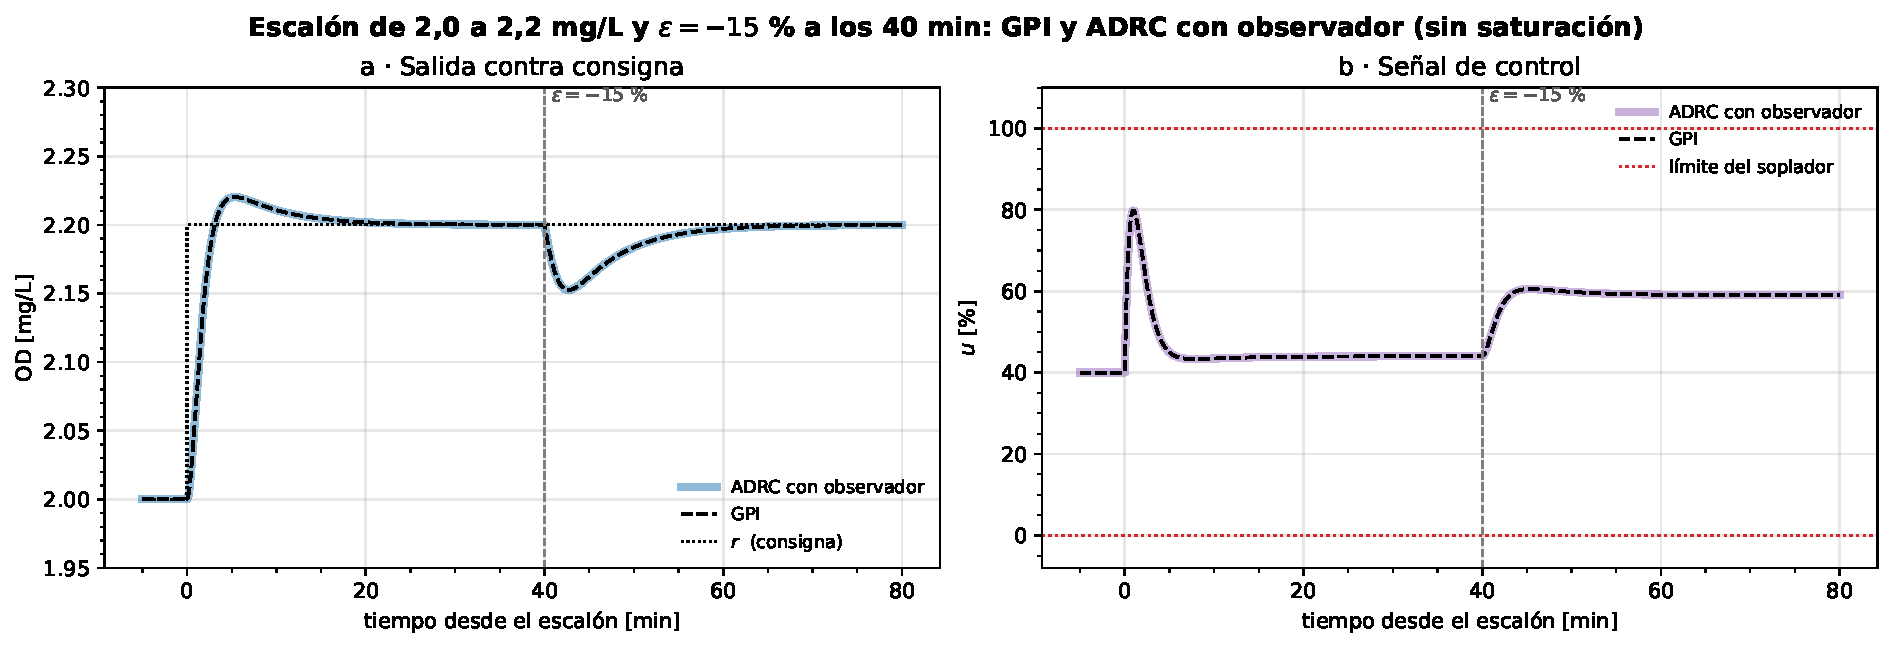
\includegraphics[width=\textwidth]{gpi_vs_adrc.pdf}
  \caption[GPI y ADRC con observador en el escalón de consigna]{Escalón de
    consigna de $2{,}0$ a $2{,}2$~mg/L y perturbación de entrada
    $\varepsilon = -15~\%$ a los $40$~min, con la planta nominal sin retardo ni
    saturación: GPI \eqref{eq:gpi_pi_filtro} y ADRC con observador
    (Sección~\ref{subsec:caso_simulacion}). (a) Salida. (b) Señal de control.}
  \label{fig:gpi_vs_adrc}
\end{figure}

Con retardo en la planta, la Figura~\ref{fig:gpi_perturbacion_retardo} repite la
entrada de la perturbación $\varepsilon = -15~\%$ con el OD en $2{,}0$~mg/L, para
$\theta$ de $0$ a $60$~s. El retardo sí afecta el rechazo: el OD baja un poco más,
de $1{,}95$ a $1{,}93$~mg/L con $60$~s, y aparece una pequeña oscilación que se
amortigua, pero la perturbación se sigue rechazando adecuadamente y la señal de
control no llega a saturarse.

\begin{figure}[H]
  \centering
  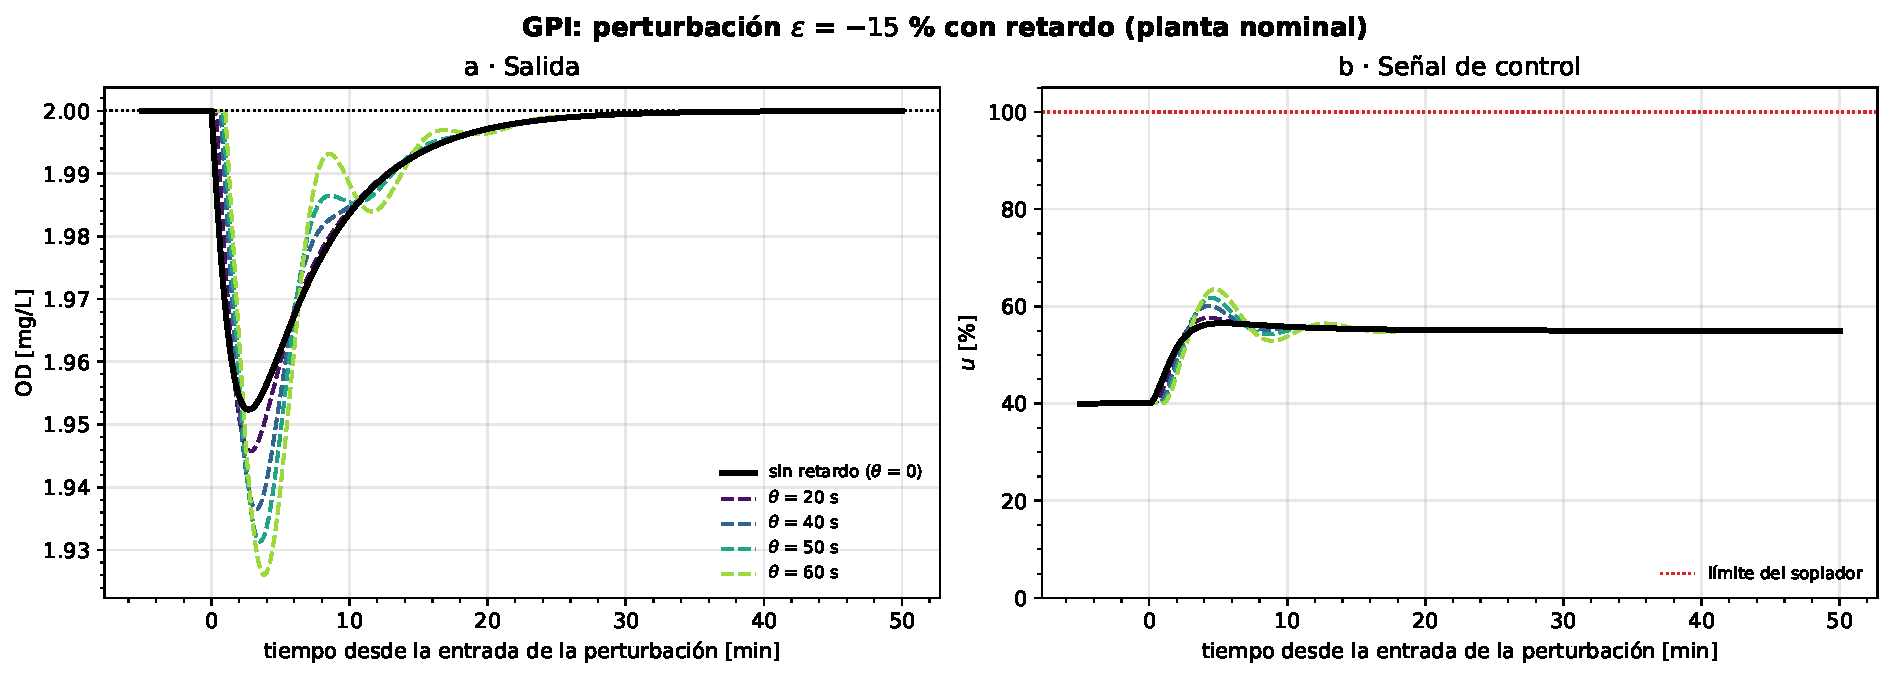
\includegraphics[width=\textwidth]{gpi_perturbacion_retardo.pdf}
  \caption[Rechazo de la perturbación con retardo con el GPI]{Entrada de una
    perturbación $\varepsilon = -15~\%$ con el OD en régimen en $2{,}0$~mg/L y la
    planta nominal con retardo $\theta$, con el GPI; en negro, sin retardo.
    (a) Salida. (b) Señal de control.}
  \label{fig:gpi_perturbacion_retardo}
\end{figure}

%--------------------------------------------------------------------
\subsection{Variación de las ganancias en el tiempo}
\label{subsec:gpi_caso_tiempo}

Para validar su comportamiento, se repite el escalón de consigna de $2{,}0$ a
$2{,}2$~mg/L, con la planta cerca del punto de operación y $u = 40~\%$, variando
cada ganancia de $1/4$ a $4$ veces su valor nominal, una a la vez y sin
saturación (Figura~\ref{fig:gpi_variacion}). El GPI se comporta como un PI con
filtro:
\begin{itemize}
  \item \textbf{$k_0$, la integral}, amplifica o disminuye el sobrepico: al
  subirla el sobrepico crece, hasta $40~\%$ con $4\,k_0$, y al bajarla
  desaparece.
  \item \textbf{$k_1$, la proporcional}, cambia el tiempo de asentamiento y las
  oscilaciones: al bajarla la respuesta oscila y tarda más en asentarse, y al
  subirla se asienta en pocos minutos, a costa de una señal de control que pasa
  del $100~\%$.
  \item \textbf{$k_2$}: al subirla, el transitorio tiene una respuesta más lenta y
  pide menos señal de control; al bajarla, el controlador es más agresivo y el
  sobrepico crece, porque además el polo del filtro se acerca al cruce de
  ganancia y le quita fase.
\end{itemize}
La Tabla~\ref{tab:gpi_transitorio} es el resumen de todo lo relacionado con las
variaciones de $k_0$ a $k_2$: sobrepico $M_p$, tiempo de asentamiento $t_s$, IAE y pico de la señal de
control (Tabla~\ref{tab:metricas}).

\begin{figure}[H]
  \centering
  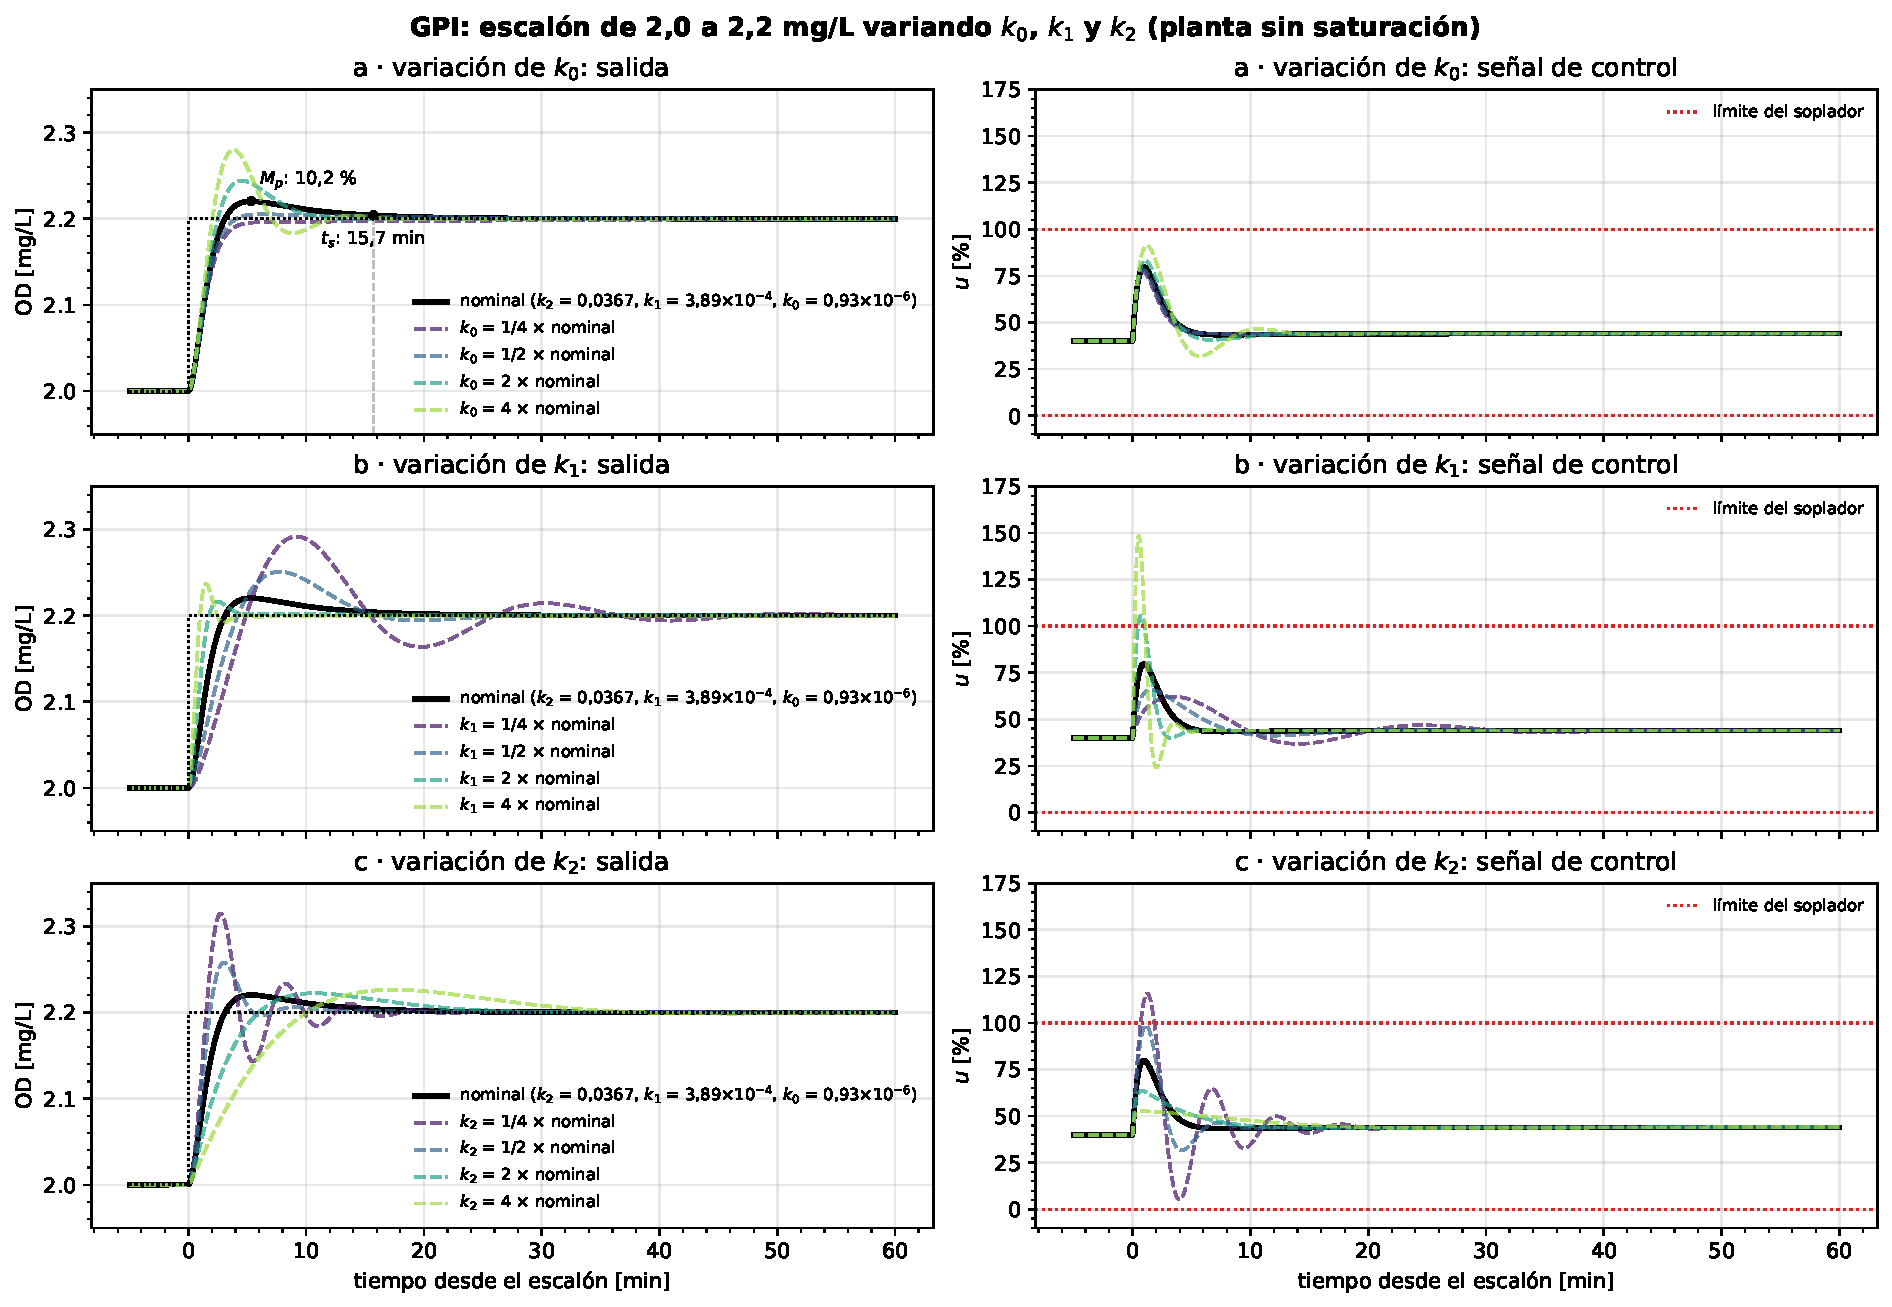
\includegraphics[width=\textwidth]{gpi_variacion_ganancias.pdf}
  \caption[Escalón de consigna con variación de las ganancias del GPI]{Escalón
    de consigna de $2{,}0$ a $2{,}2$~mg/L con el GPI y la planta, variando
    (a) $k_0$, (b) $k_1$ y (c) $k_2$. Izquierda, la salida; derecha, la señal
    de control. En negro, las ganancias nominales de la Tabla~\ref{tab:gpi_eso}.}
  \label{fig:gpi_variacion}
\end{figure}

\begin{table}[H]
\centering
\caption[Resumen del transitorio del GPI al variar sus ganancias]{Resumen del
transitorio del escalón de $2{,}0$ a $2{,}2$~mg/L de la
Figura~\ref{fig:gpi_variacion} al variar $k_0$, $k_1$ y $k_2$.}
\label{tab:gpi_transitorio}
\small
\begin{tabular}{llrrrr}
\toprule
\textbf{Ganancia} & \textbf{Factor} & $M_p$ [\%] & $t_s$ [min] & IAE [mg$\cdot$min/L] & $u_{\max}$ [\%] \\
\midrule
nominal & $1$    & $10{,}2$  & $15{,}7$  & $0{,}448$ & $79{,}8$ \\
\midrule
$k_0$   & $1/4$  & $0{,}0$   & $5{,}9$   & $0{,}423$ & $77{,}4$ \\
        & $1/2$  & $2{,}6$   & $10{,}4$  & $0{,}382$ & $78{,}2$ \\
        & $2$    & $22{,}2$  & $10{,}4$  & $0{,}458$ & $83{,}3$ \\
        & $4$    & $40{,}1$  & $11{,}3$  & $0{,}531$ & $91{,}2$ \\
\midrule
$k_1$   & $1/4$  & $45{,}9$  & $43{,}6$  & $1{,}531$ & $62{,}1$ \\
        & $1/2$  & $25{,}4$  & $22{,}4$  & $0{,}796$ & $65{,}8$ \\
        & $2$    & $8{,}2$   & $4{,}0$   & $0{,}233$ & $105{,}7$ \\
        & $4$    & $18{,}4$  & $3{,}6$   & $0{,}171$ & $148{,}4$ \\
\midrule
$k_2$   & $1/4$  & $57{,}3$  & $16{,}8$  & $0{,}604$ & $115{,}9$ \\
        & $1/2$  & $28{,}8$  & $10{,}6$  & $0{,}368$ & $98{,}7$ \\
        & $2$    & $11{,}1$  & $23{,}1$  & $0{,}722$ & $63{,}6$ \\
        & $4$    & $13{,}2$  & $33{,}1$  & $1{,}229$ & $52{,}8$ \\
\bottomrule
\end{tabular}
\end{table}

%--------------------------------------------------------------------
\subsection{Sensibilidad en lazo cerrado}
\label{subsec:gpi_caso_sensibilidad}

Para ver el efecto de las ganancias en frecuencia se usa la función de
sensibilidad en lazo cerrado frente a la perturbación total,
$e_y(s) = S_{\xi}(s)\,\xi(s)$ \eqref{eq:gpi_S}. Con los valores de la
Tabla~\ref{tab:gpi_eso},
\begin{align}
S_{\xi}(s) &= \frac{s\,(s + k_2)}{s^3 + k_2 s^2 + k_1 s + k_0}
= \frac{s\,(s + 0{,}0367)}{s^3 + 0{,}0367\,s^2 + 3{,}89\times10^{-4}\,s + 9{,}26\times10^{-7}} \nonumber\\[4pt]
&= \frac{s\,(s + 0{,}0367)}{(s + 0{,}00333)\,(s + 0{,}0167)^2} ,
\label{eq:gpi_caso_S}
\end{align}
cuyo denominador tiene los polos de diseño, en $-\omega_c$ y $-\omega_o$; con la
planta nominal el lazo cerrado los mueve un poco (Tabla~\ref{tab:caso_polos}),
pero $S_{\xi}$ no cambia, porque esa diferencia queda dentro de $\xi$.
\begin{equation}
S_{\xi}(s) \xrightarrow{\;s\to 0\;} \frac{k_2}{k_0}\,s ,
\qquad
S_{\xi}(s) \xrightarrow{\;s\to \infty\;} \frac{1}{s} .
\label{eq:gpi_caso_S_asintotas}
\end{equation}
A baja frecuencia $S_{\xi}$ crece como $(k_2/k_0)\,s$: el integrador del
controlador rechaza las perturbaciones lentas, y entre más pequeño sea
$k_2/k_0$, mejor las rechaza. A alta frecuencia tiende a $1/s$, una integral,
que es lo mismo que pasaría sin control: perturbaciones tan rápidas el
controlador ya no las alcanza a compensar, y solo las suaviza la planta. Entre
más baja esté la curva, mejor se rechaza la perturbación; $S_{\xi}$ no habla del
ruido del sensor, que entra por la medida y llega al soplador por otra función
del lazo (Figura~\ref{fig:adrc_gang_kESO}(h)). En la
Figura~\ref{fig:gpi_sensibilidad} se ve que:
\begin{itemize}
  \item con $k_0$ y $k_2$ se sube o se baja la curva a baja frecuencia: subir
  $k_0$ o bajar $k_2$ la baja y rechaza mejor las perturbaciones lentas, y lo
  contrario la sube;
  \item con $k_1$ se mueve el pico central, el de resonancia: al bajar $k_1$ el
  pico crece y la perturbación se amplifica cerca de esa frecuencia, y al
  subirlo el pico baja y se corre a frecuencias más altas.
\end{itemize}

\begin{figure}[H]
  \centering
  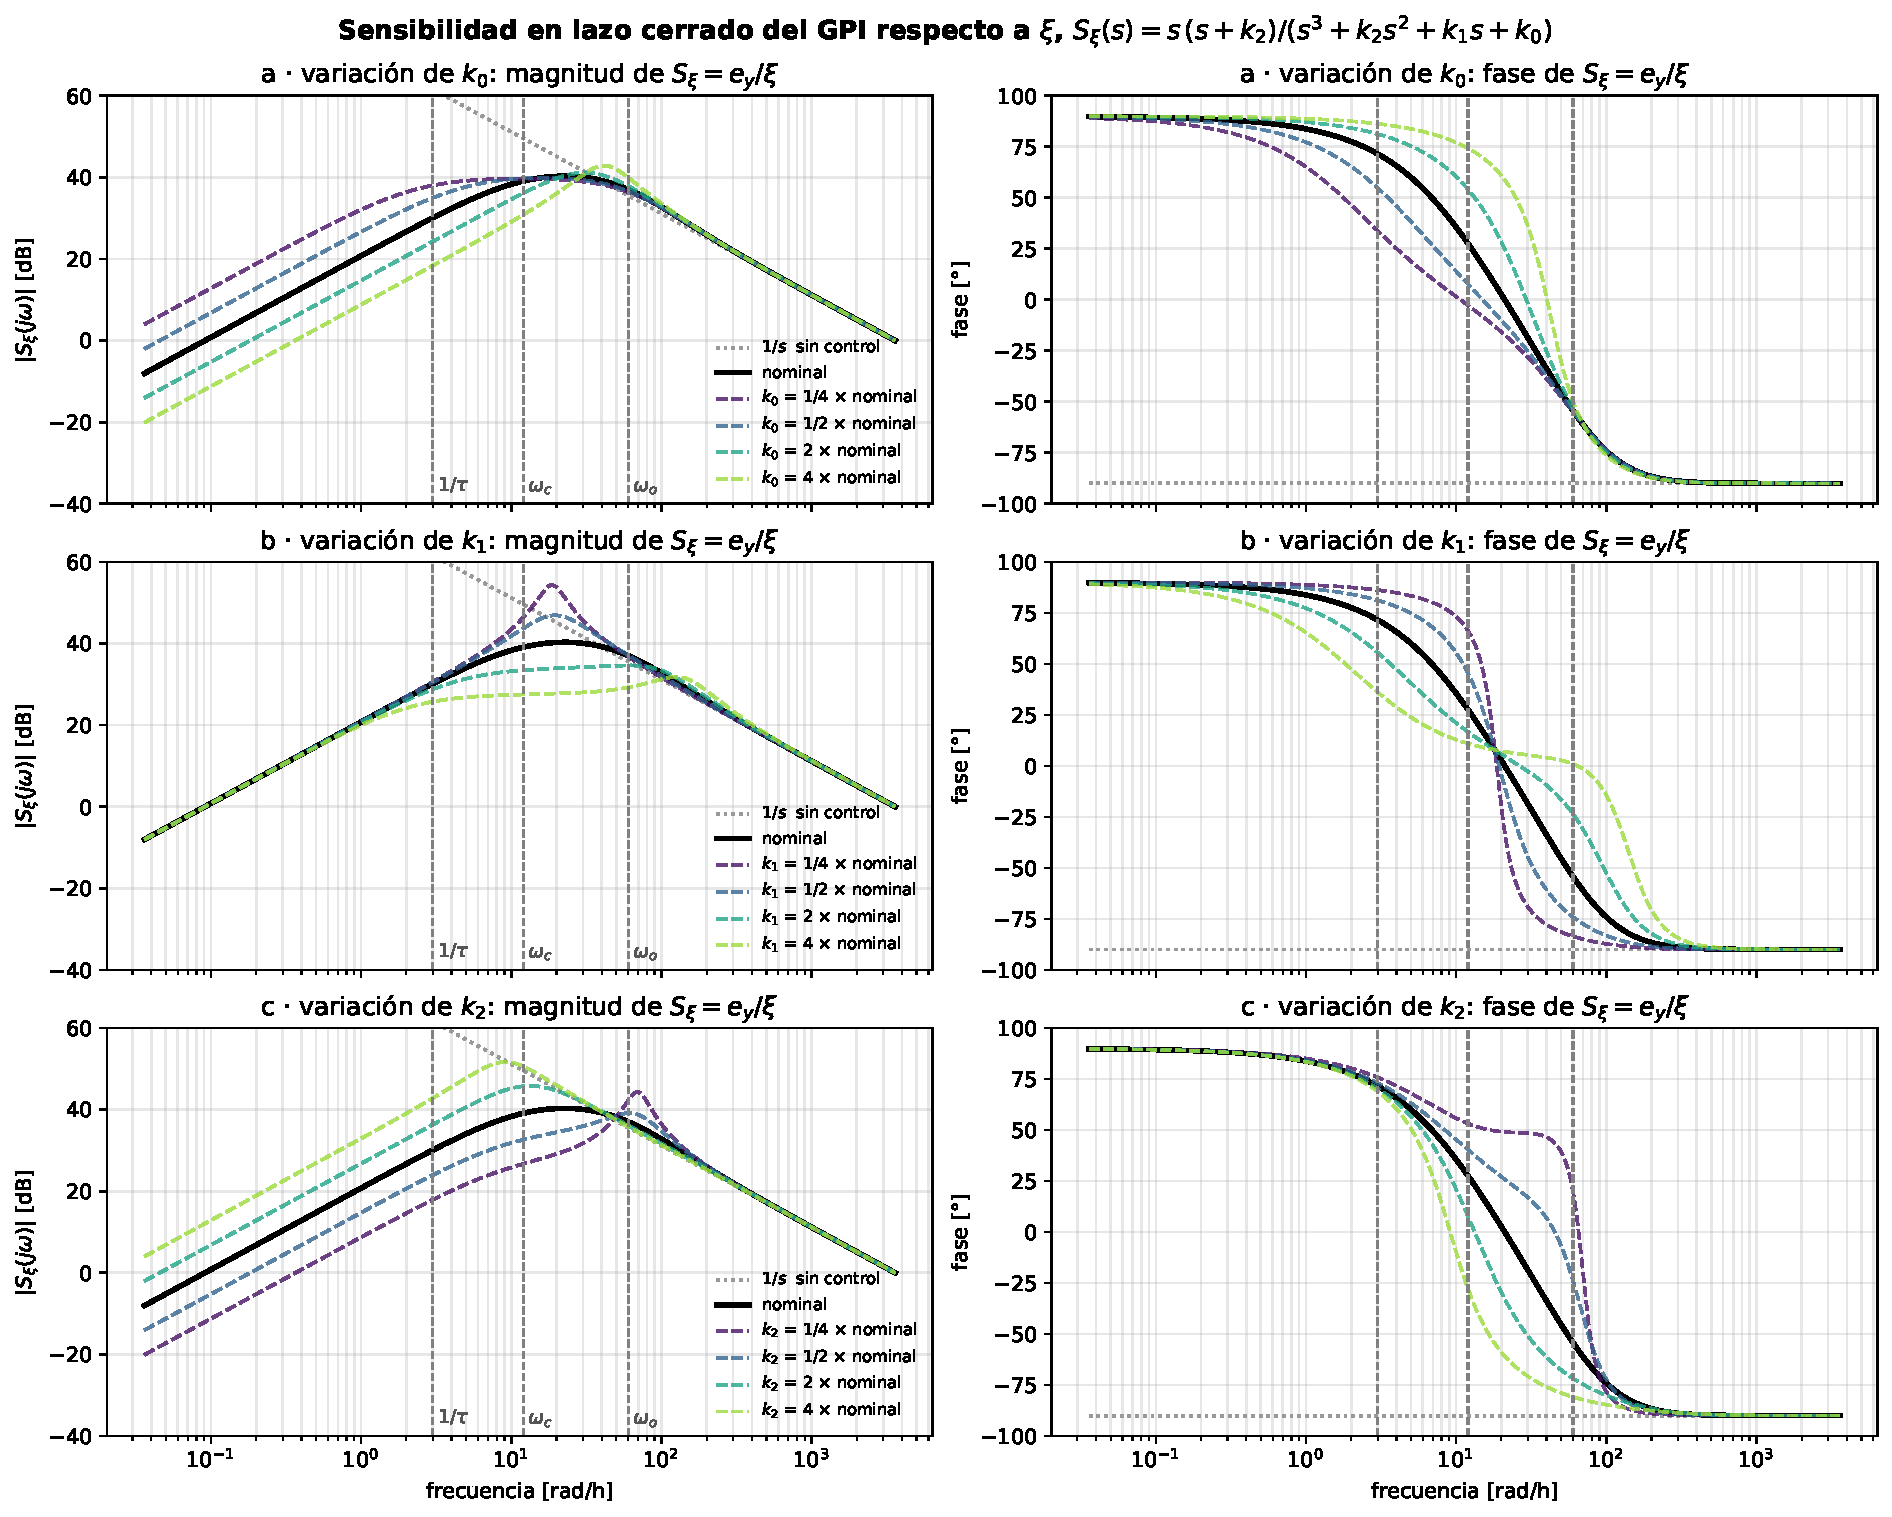
\includegraphics[width=\textwidth]{gpi_sensibilidad.pdf}
  \caption[Sensibilidad en lazo cerrado del GPI al variar sus ganancias]{Bode
    de la sensibilidad en lazo cerrado $S_{\xi}(s) = e_y/\xi$ \eqref{eq:gpi_caso_S},
    variando (a) $k_0$, (b) $k_1$ y (c) $k_2$; $\xi$ en mg/(L$\cdot$s), así que
    $|S_{\xi}|$ está en dB respecto a $1$~s. Izquierda, magnitud; derecha, fase. En
    gris punteado, $1/s$, el error sin control; las verticales marcan $1/\tau$,
    $\omega_c$ y $\omega_o$.}
  \label{fig:gpi_sensibilidad}
\end{figure}


Para ver cómo cambia la robustez con cada ganancia, la
Figura~\ref{fig:gpi_margen_fase} muestra el lazo abierto $C(s)\,G(s)$ con la
planta nominal al variar $k_0$, $k_1$ y $k_2$, con el margen de fase de cada caso.
Lo que se gana en rechazo se pierde en robustez, y se debe llegar siempre a un
equilibrio: subir $k_0$ le quita fase cerca del cruce de ganancia, y subir $k_1$ o
bajar $k_2$ lleva el cruce a frecuencias más altas; en los dos casos el margen de
fase y el retardo que aguanta el lazo tienden a bajar. Con $k_2/4$, por ejemplo, el margen
cae a unos $21^{\circ}$ y el lazo solo aguanta unos $20$~s de retardo, menos que
los $50$~s de la planta. Bajar $k_1$ tampoco ayuda, porque el pico de resonancia
que crece también le quita margen. Subir $k_2$ hace lo contrario: más margen y
más retardo tolerable, pero peor rechazo de las perturbaciones.

Estas relaciones no siempre se cumplen, porque dependen de dónde quede la frecuencia de cruce de
ganancia y de cómo se comporte la fase. Lo mejor es disminuir $k_0$, para tener un sistema más lento
y ganar margen de fase, sintonizar $k_2$ a partir del ruido que se desea filtrar, y siempre validarlo
con simulación. La Tabla~\ref{tab:gpi_frecuencia} resume las Figuras~\ref{fig:gpi_sensibilidad}
y~\ref{fig:gpi_margen_fase}.

\begin{figure}[H]
  \centering
  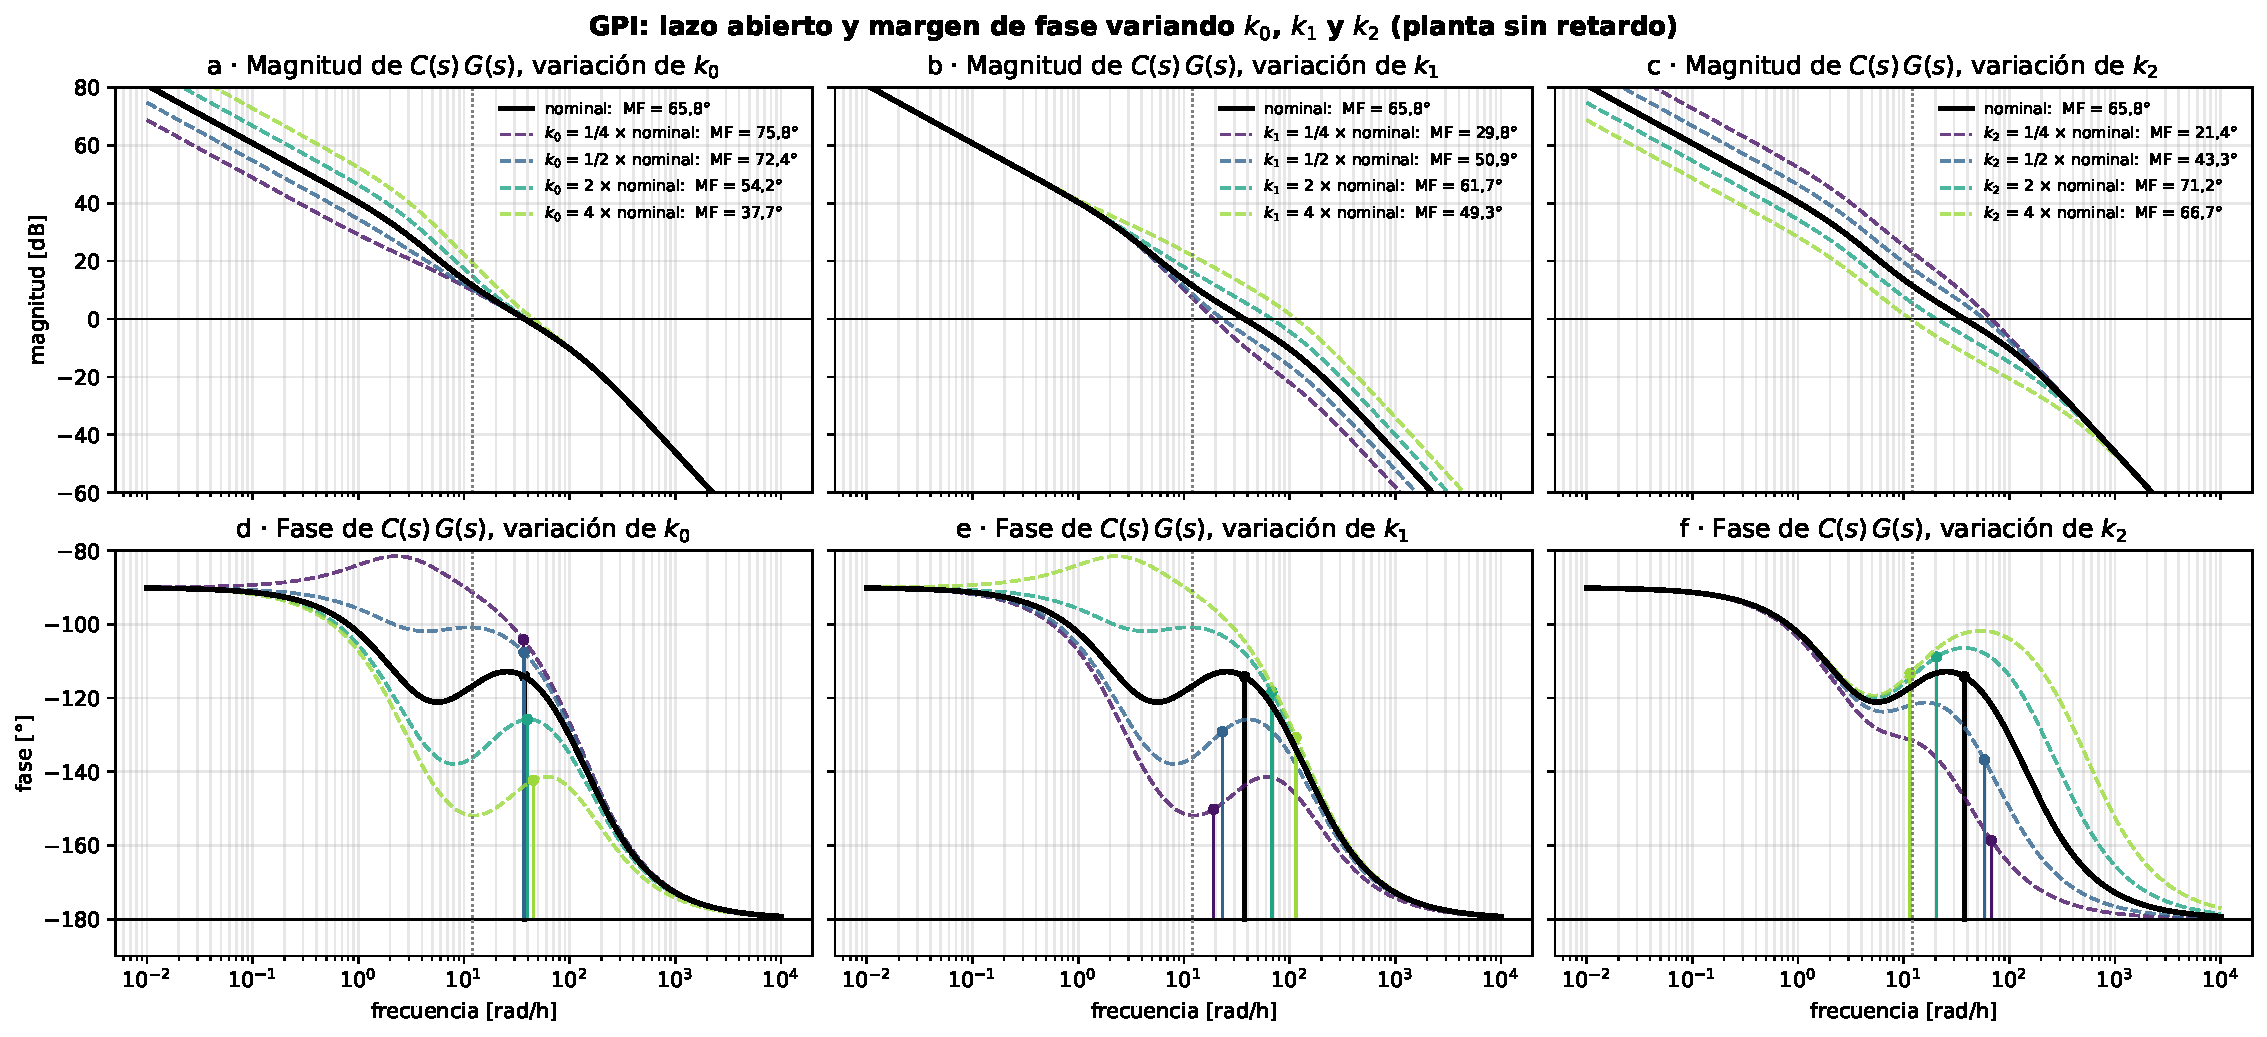
\includegraphics[width=\textwidth]{gpi_margen_fase.pdf}
  \caption[Margen de fase del GPI al variar sus ganancias]{Lazo abierto
    $C(s)\,G(s)$ con la planta nominal sin retardo, variando (a, d) $k_0$,
    (b, e) $k_1$ y (c, f) $k_2$; en negro, las ganancias nominales. Arriba, la
    magnitud; abajo, la fase, con el margen de fase como segmento vertical y su
    valor en la leyenda. La vertical punteada marca $\omega_c$.}
  \label{fig:gpi_margen_fase}
\end{figure}

\begin{table}[H]
\centering
\caption[Sensibilidad y robustez del GPI al variar sus ganancias]{Resumen de
  las Figuras~\ref{fig:gpi_sensibilidad} y~\ref{fig:gpi_margen_fase}: pico de
  $|S_{\xi}| = |e_y/\xi|$ \eqref{eq:gpi_caso_S} y su frecuencia, pendiente $k_2/k_0$
  a baja frecuencia \eqref{eq:gpi_caso_S_asintotas}, y margen de fase, retardo
  máximo y $M_s$ del lazo con la planta nominal sin retardo,
  variando una ganancia a la vez.}
\label{tab:gpi_frecuencia}
\small
\begin{tabular}{llrrrrrr}
\toprule
\textbf{Ganancia} & \textbf{Factor} & pico $|S_{\xi}|$ [dB] & en [rad/h] & $k_2/k_0$ [h] & MF [°] & $\theta_{\max}$ [s] & $M_s$ \\
\midrule
nominal & $1$ & $40{,}3$ & $22{,}6$ & $11{,}0$ & $65{,}8$ & $110$ & $1{,}202$ \\
\midrule
$k_0$ & $1/4$ & $39{,}7$ & $11{,}7$ & $44{,}0$ & $75{,}8$ & $130$ & $1{,}171$ \\
 & $1/2$ & $39{,}9$ & $16{,}3$ & $22{,}0$ & $72{,}4$ & $123$ & $1{,}180$ \\
 & $2$ & $41{,}1$ & $30{,}8$ & $5{,}5$ & $54{,}2$ & $86$ & $1{,}271$ \\
 & $4$ & $42{,}9$ & $41{,}5$ & $2{,}8$ & $37{,}7$ & $52$ & $1{,}608$ \\
\midrule
$k_1$ & $1/4$ & $54{,}3$ & $18{,}6$ & $11{,}0$ & $29{,}8$ & $98$ & $1{,}977$ \\
 & $1/2$ & $46{,}9$ & $19{,}5$ & $11{,}0$ & $50{,}9$ & $138$ & $1{,}240$ \\
 & $2$ & $34{,}6$ & $60{,}6$ & $11{,}0$ & $61{,}7$ & $57$ & $1{,}313$ \\
 & $4$ & $31{,}8$ & $125{,}4$ & $11{,}0$ & $49{,}3$ & $27$ & $1{,}516$ \\
\midrule
$k_2$ & $1/4$ & $44{,}3$ & $69{,}1$ & $2{,}8$ & $21{,}4$ & $20$ & $2{,}865$ \\
 & $1/2$ & $39{,}1$ & $61{,}0$ & $5{,}5$ & $43{,}3$ & $47$ & $1{,}627$ \\
 & $2$ & $45{,}8$ & $13{,}3$ & $22{,}0$ & $71{,}2$ & $219$ & $1{,}062$ \\
 & $4$ & $51{,}7$ & $9{,}1$ & $44{,}0$ & $66{,}7$ & $364$ & $1{,}023$ \\
\bottomrule
\end{tabular}
\end{table}


